\documentclass{book}

\usepackage{standalone} % Must be loaded early
\usepackage{hyperref}
\usepackage{graphicx}
\usepackage{minted}
\usepackage{currfile}
\usepackage{graphviz}
\usepackage{tikz}
\usepackage{pdflscape}

\title{minigrep \\ \large{System Requirements and Specification}}
\author{Alex G. Ramirez}
\date{April 18th, 2026}

\begin{document}
\maketitle
\tableofcontents

\chapter{Abstract}

This document contains the specifications (requirements, user stories, Gherkin 
features, unit tests, and integration tests) for the minigrep application defined
in the \href{https://doc.rust-lang.org/book/ch12-00-an-io-project.html}
{Rust Language Book: Chapter 12}\footnote{\url{https://doc.rust-lang.org/book/ch12-00-an-io-project.html}}.

The document also provides the design and implementation details for the project.
\begin{quotation}
    NOTE: The design and implementation will differ from the vanilla implementation
    as defined in the Rust Language Book.  The reason for this is to use and showcase
    some advanced documentation and testing features.
\end{quotation}

\section{Sections}

This docuemnt will be split into the following sections, each will be described in
detail:

\begin{itemize}
    \item Ideas
    \item Requirements
    \item Design
\end{itemize}

\subsection{Ideas}
The \emph{Ideas} section will contain general ideas, notes, and general info that
will drive the requirements, features, design, tests, etc.  It will be useful for
context regarding requirements and design decisions.

\begin{quotation}
    NOTE\: For the purposes of this document we will mainly use references to the
    Rust Book Chapter 12 minigrep project.
\end{quotation}

Each \emph{Idea} subsection will have a corollary subsection in the \emph{Requirements}
and \emph{Design} sections.  This will reflect the Software Development Lifecycle (SDLC)
process.

\subsection{Requirements}
The \emph{Requirements} section will contain Gherkin feature stories simulating
direct requirements gathering from stakeholders.  These features will be used
in integration tests using the Rust cucumber package.

Once all of the features are implemented the code will be considered ready for 
production.

Note that special emphasis is placed on this specific section and most of the 
processes, tools, and examples will be geared towards this section.

An Agile development approach will be considered as the primary method of 
development with Behaviour Driven Development and Test Driven Development
being at the forefront of the process.

The tight integration of User Defined Features via Gherkin, automated testing
tools like Cucumber and Erlang's Common Test framework will ensure that development
time and budgets are efficiently and correctly utilized for maximum client
satisfaction\footnote{Yes, this is a bit of a cheeky statement, but it is true enough}! \:P

\subsection{Design}
The \emph{Design} section will provide general implementation details in the 
form of UML Component and Communication diagrams.  Optionally, we might include
User Story diagrams as well, but these will essentially be visual versions of 
the Gherkin scenarios.

Of special note, our design will focus on implementing a solid BDD and TDD 
framework for our initial Proof of Concept (POC) and Minimum Viable Product 
(MVP) stages of our features.

Security\footnote{Examples include input validation, authentication, and authorization, etc.}, 
visibility\footnote{Examples include logging, metrics, tracing, etc.}, 
scalability\footnote{Examples include gateway implementation, eventual consistancy algorithms, etc.}, 
availability\footnote{Examples include backups, database sharding, etc.}, and 
performance\footnote{Examples include implementing algorithms to minimize memory and CPU consumption} will be 
considered as separate and incremental stages in our implementation.
This will provide a solid base for Agile development of features and 
functionality while maintaining focus on enterprise grade software that can safely
and efficiently scale from dozens to millions of users.

\subsection{Ommitted Sections}
In a production environment we would also like to create a backlog of features
to be implemented in an Agile style.  This section would be called \emph{Implementation}
and would include details like the developers who are assigned the work, the 
Agile story points, schedules, etc.

Another ommitted section will be the \emph{Deployment} section.  This section
provides information about the actual features deployed, version control info,
and many other deployment details like environment infrastructure information
(ie servers, ips, tech stack, etc.) 

\chapter{Idea}

\section{Accepting Command Line Arguments}

In this section\footnote{\url{https://doc.rust-lang.org/book/ch12-01-accepting-command-line-arguments.html}}
we implement functionality to get the command line variables provided to the \emph{minigrep} application.

We have codified this requirement in the \hyperref[call_feature]{call.feature}.

\chapter{Requirements}

\section{Accepting Command Line Arguments}

\subsection{Features}

\inputminted{gherkin}{../features/call.feature}\label{call_feature}

\chapter{Design}
\begin{minipage}{\textwidth}
\section{Accepting Command Line Arguments}
The diagram below shows the general communication flow for the command line 
arguments feature.  Note that the primary features are described as 

\begin{itemize}
    \item Dependency Injection
    \item File Access
    \item Search Success
    \item File Access Error
\end{itemize}

This segregation of responsibilities should be reflected in the objects, 
classes, components, and threads implemented from this design.  The next 
diagrams show how the components should be structued and how the classes
should relate to each other.

\makebox[\textwidth][c]{
    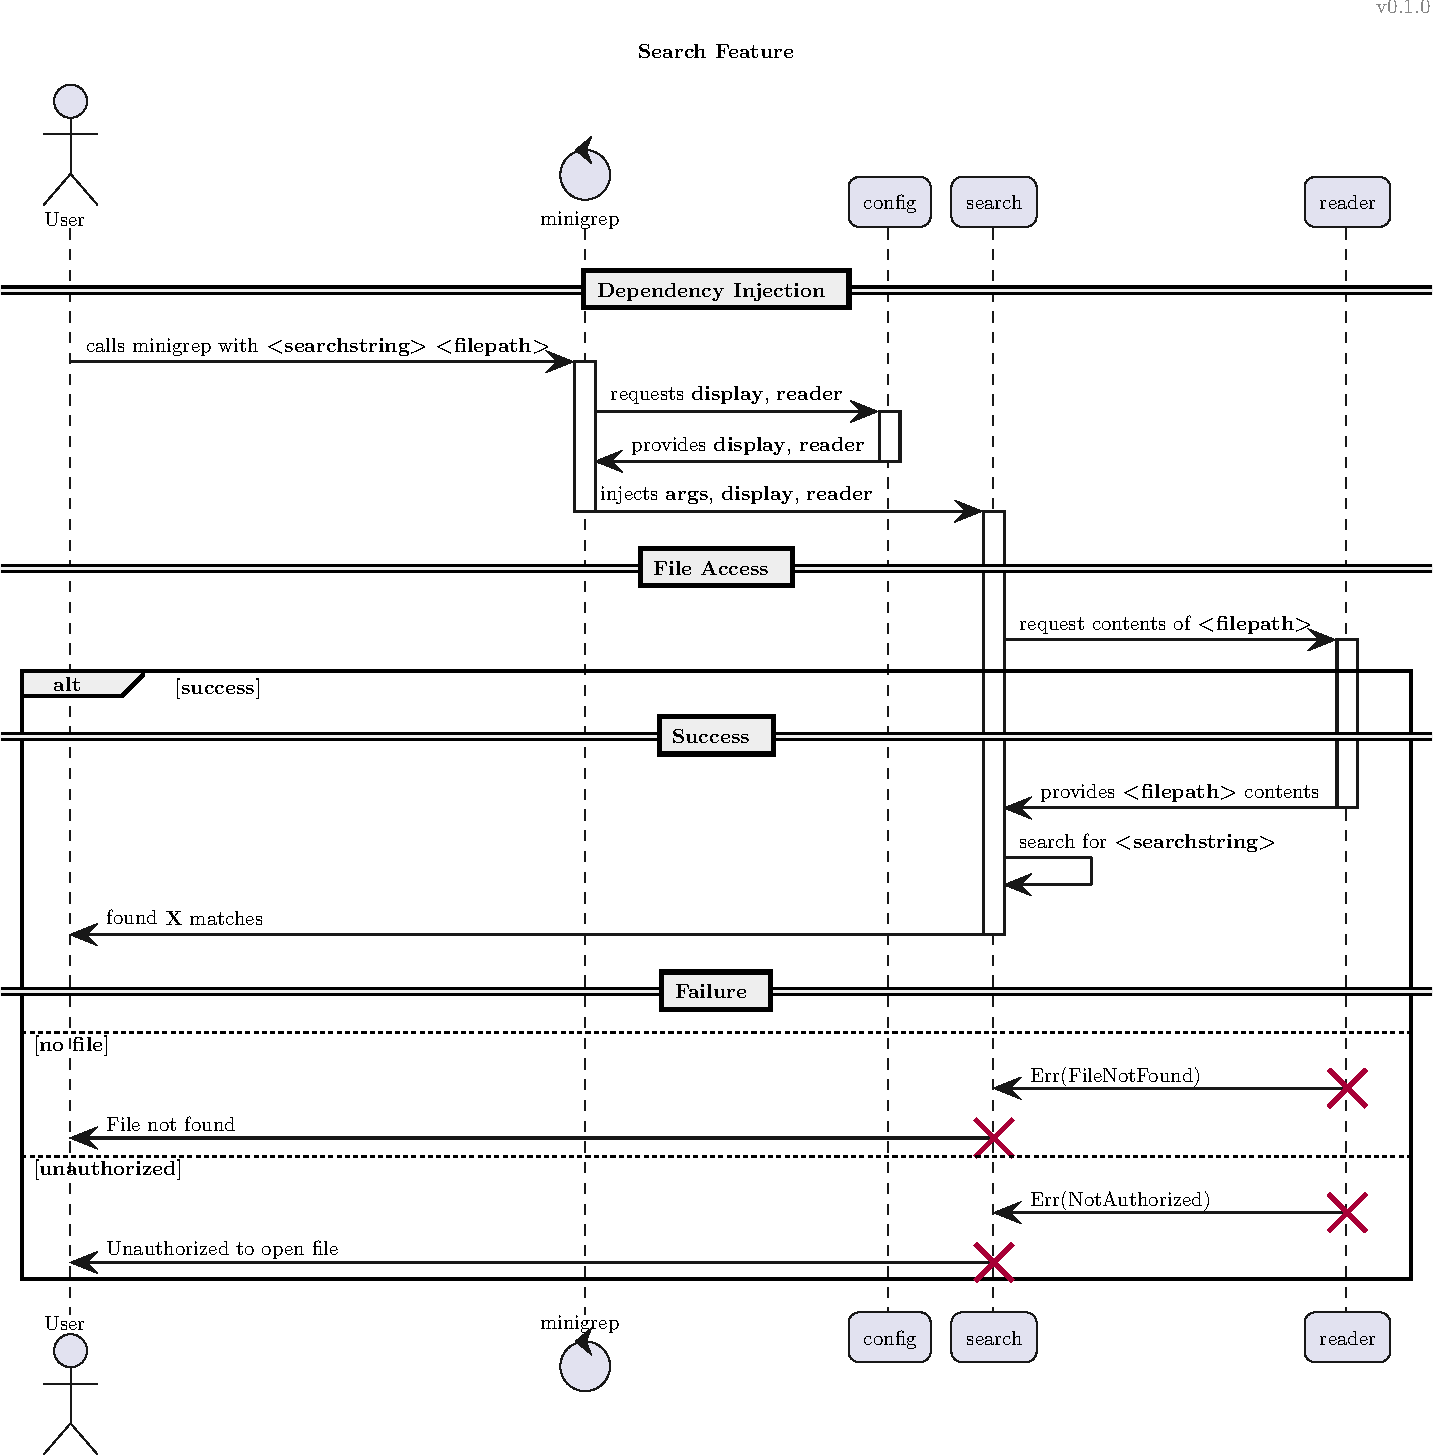
\includegraphics[width=1.1\textwidth,keepaspectratio]{./call_feature/call_feature.pdf}
}
\end{minipage}

\subsection{Design Rationale}

The reason why the design is clearly deliniated into the four components
is to ensure testability by providing clear demarcation of dependency injection
architecture, segmenting environment access (config, file read, and message output)
for the same, and ensuring that the implemented design follows these architectural
best practices.

\begin{quotation}
    NOTE\: Security and logging will be considered in future iterations of the design.
    They were not implemented to provide an example of iterative development practices 
    that begin with a Proof Of Concept, move to a Minimum Viable Product, and progressively 
    enhance maintainability, scalability, and code performance.

    However, without a solid DI and TDD framework it would not be possible to efficiently 
    implement this incremental enhancement process.
\end{quotation}

\end{document}